\section{APR}
\subsection{APR 是什么}
首先请看官方说明。没看过的同学,请务必逐字逐句阅读完毕,因为APR重要性相当于一次小答辩。不通过的,会被退学。

\url{https://www.liverpool.ac.uk/student-administration/research-students/progression/annual-progress/}

在我的理解里,APR的作用是
\begin{itemize}
    \item Interview: 读PhD本身很不容易,所以学校、学院需要了解学生遇到的问题,帮助解决
    \item Seminar: 锻炼作报告的能力 + 认识其他博士生同学
    \item Progress report: 检查学生进度,进一步发现并帮助解决学生遇到的问题。同时,筛查完全不认真学习的学生
\end{itemize}

有同学一开始面对APR的时候会很紧张。实际上,进度报告部分,只要不是一整年真的天天混日子,看书、读文献、写文章、做调查、做实验、写代码等等任何一样都没干,评审老师是不会刁难你不给过的。听说22年某学院APR有个学生不通过,据可靠消息此人是近乎人间蒸发,导师消息完全不回,工作不做,才fail的。

而且要注意到,APR的另一个主要功能是——帮助大家解决问题。所以,反而应该大胆的在APR里暴露自己的问题,寻求帮助 (Chapter. \ref{section:IPAP})。

\subsection{APR 流程}
\subsubsection{准备工作}
APR的前置任务只有一个,那就是要填完\textbf{每月至少一次}的会议记录。关于如何填写会议记录,参见章节 \ref{section:meeting_record}。

然后,每年关于APR有两封重要邮件
\begin{enumerate}
    \item 
        \begin{minipage}{0.3\textwidth}
            其一为西浦在5月发的邮件,大概长这样,发到西浦邮箱
        \end{minipage}
        \begin{minipage}{0.63\textwidth}
            \begin{figure}[H]
                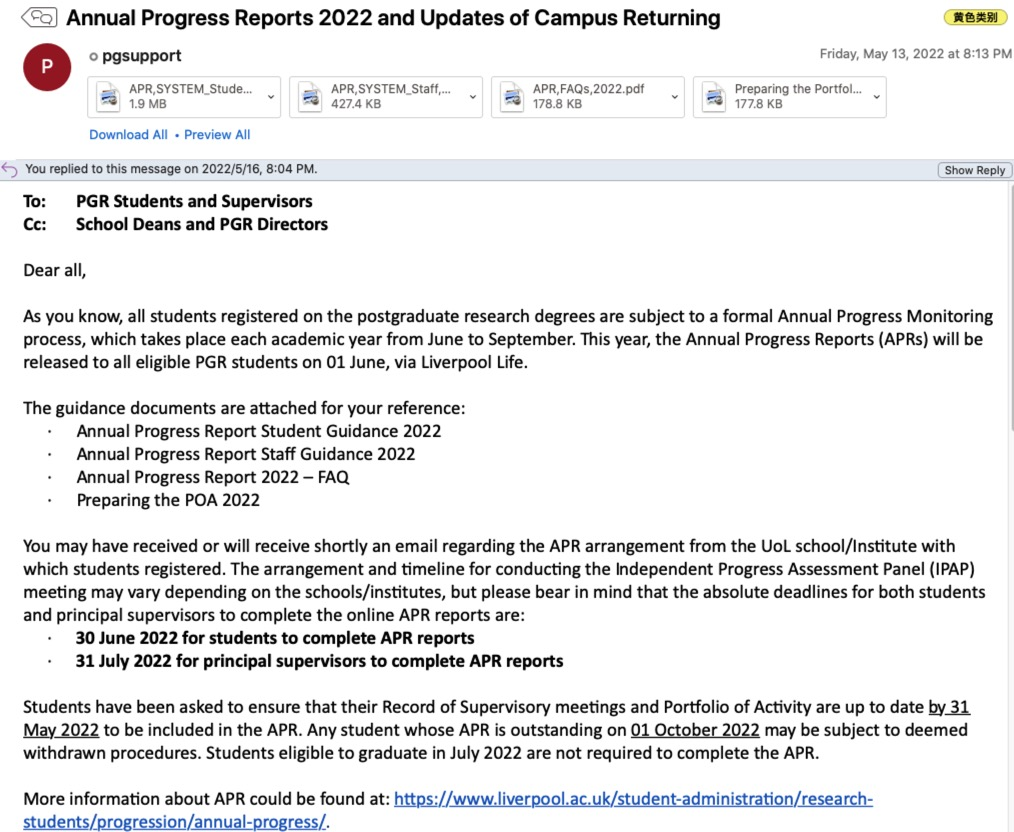
\includegraphics[width=0.95\columnwidth, right]{author-folder/Kai.Wu/APR_email.jpg}
            \end{figure}
        \end{minipage}

    \item 
        \begin{minipage}{0.3\textwidth}
            其二为你的利物浦学院在4月到5月发的邮件,数学学院的大概长这样,发到利物浦邮箱。其他学院的可能不太一样。各个学院发通知的时间也有很大不同,有4月就发的,有拖到5月底的。
        \end{minipage}
        \begin{minipage}{0.63\textwidth}
            \begin{figure}[H]
                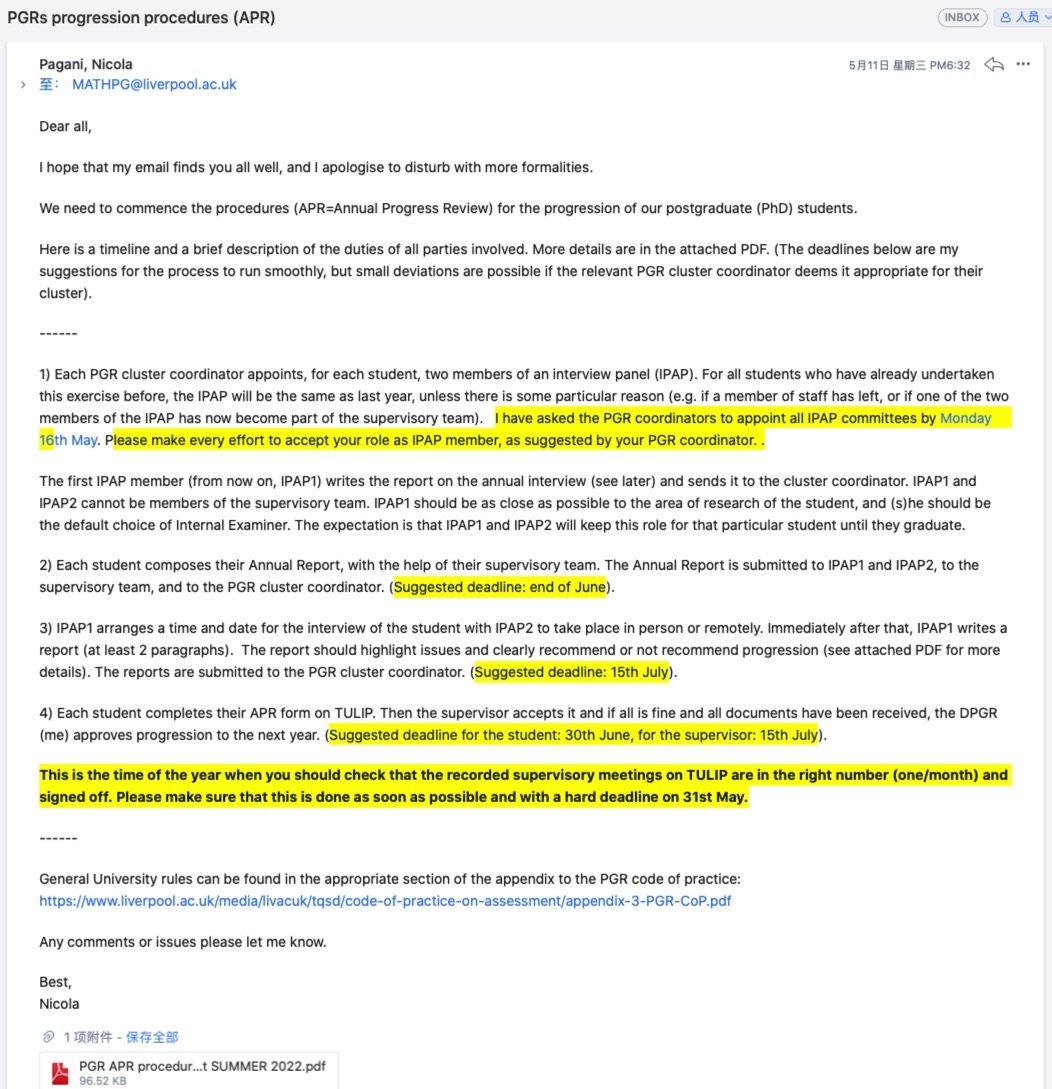
\includegraphics[width=0.95\columnwidth, right]{author-folder/Kai.Wu/APR_liverpool_email.jpg}
            \end{figure}
        \end{minipage}

\end{enumerate}

每个学院的APR要求略有区别,所以在5月左右,请务必查收你的利物浦邮箱。两封邮件,请务必仔细阅读。\textbf{初次做APR的同学,建议对两封邮件和附件,逐字阅读。}

APR的具体内容就是下面四个部分
\subsubsection{TULIP 网页表格}
利物浦和西浦邮件里所谓的 “Your annual progress report has been released" 就是说这个绿油油的表你可以填了。里面主要是这几部分要填:
\begin{enumerate}
    \item SUMMARY OF PROGRESS 进度报告,300词以上,4000字符(约600词)以下
    \item Seminars and Conference attendance, Library and IT training and all subject specific training including research methods and experimental techniques. (回忆一下,越多越好,实在没有也没关系)参加的会议、研讨会、专业技能培训
    \item Attendance at careers events and workshops covering Employability and Entrepreneurship and including attendance at any other Professional development workshops. (越多越好)参加的就业相关活动
    \item Training and completion of activities relating to Health and Safety, ethics, grant writing and similar activities, including Project Management. (越多越好)参加的和学习不直接相关但又有关的活动
    \item Details of your Presentations, written publications, teaching and public engagement/Impact activities and related training in for these activities. (越多越好)参加的展示、发表的论文、做过的助教
    \item PERSONAL OR ACADEMIC PROBLEMS: Have there been any problems in the last year which you feel have affected your progress? (按实际情况填写)有没有遇到什么阻碍学习的问题。直白点说,可以真切的提出问题,也可适当甩锅,就是“我进度不够都是因为xxxxxx(生病了/结婚了/学校网络不行/自己英语阅读太慢/自己某方面能力欠缺)”
\end{enumerate}

\begin{figure}[H]
    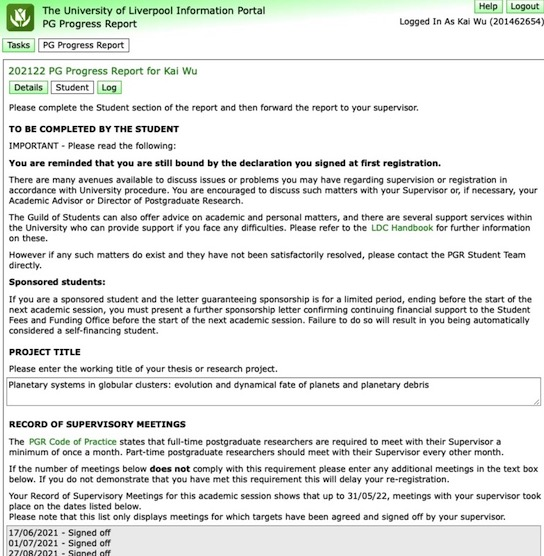
\includegraphics[width=0.7\columnwidth, center]{author-folder/Kai.Wu/TULIP.jpg}
\end{figure}

TULIP表不分学院,所有同学都肯定要填。但以下 ↓ 三个部分\textbf{各个学院要求可能非常不同,同时还部分取决于你隶属的利物浦学院},可能跟你的学长学姐double check。

\subsubsection{Annual Report (AR) 年度报告}
简单来说,把你做了什么\textbf{写成一篇文档}。一般会有字数或者页数要求。如果你真的不知道写什么,我个人建议可以事无巨细的写,按时间顺序\sout{(写成流水账)},比如,读了什么文献,有了什么收获;写了什么代码/做了什么实验。以及很重要的,参加了什么学术活动,比如参加conference, meeting,还有做学校的TA,都可以写进去。换而言之,就是把上面的TULIP表格的内容用文档再说一遍,基本就是复制粘贴,然后字数不够的话扩充一下内容。

当然,有特殊要求的按要求做,比如数学学院对 Year 3 要求交 Thesis Outline 毕业论文大纲就可以,那就不用写流水账了。

请注意,这部分AR的描述是以我所在的数理学院为例。听其他学院同学说,很多学院要求是类似的,但也有学院要求超级多。据某化学专业同学,他们第一年要写30-50页文献综述,这种就必须提前一两个月开始准备。\textbf{新同学请务必咨询你的学长学姐或者导师。}

\subsubsection{Annual Seminar 年度研讨会}
一般是把一个学院或者一个系的所有PhD拉到一起做个展示,互相提提意见,了解下。但据我所知,有的人少的系直接跳过了这一部分,或者把这一部分融合到下面的面试里,变成给两位老师讲。不管是什么形式,你需要\textbf{做一个PPT},让别人了解你的研究。时长可以按20分钟展示+5分钟提问准备,有些学院要求可能不一样,问学长学姐。如果你工作成果多,可以挑重点展示;如果不多的话,流水账一样展示自己做了什么,撑起来时长,让老师觉得你做了很多工作就行。

\subsubsection{IPAP Interview 面试}
\label{section:IPAP}
学院会找两位不是你的导师且和你没有利益冲突的老师来和你面谈。你可能需要\textbf{做一个PPT},在里面放心大胆写下你遇到的问题。由于你的导师团队被禁止接触这一部分,所以你可以畅所欲言,以下问题都可以和IPAP老师谈。按照要求,两位老师会竭尽所能帮你解决问题
\begin{itemize}
    \item 设备问题:学校电脑故障,比如哪里用起来不顺手,卡顿,死机;办公室环境问题(例如空调对着头吹)
    \item 实实在在的科研问题:你文献读得太少,但又不知道怎么高效读;你不知道实验方法;你写作有很大困难;你因为非主观的原因无法参加很多学术会议(比如这几年,每年APR我们都要吐槽疫情的各种影响)等等
    \item 导师问题:你导师压榨你,每天让你996工作,让你疲惫不堪;你导师让你做很多无关工作,比如给他搬家,给他拿外卖,给他报销;你导师对你很凶,对你很push,让你每天精神高度紧张;你导师频繁在非工作时间打电话、发微信、邮件并要求你立即回复,让你无法休息;你导师抢你论文一作;你导师长期失联,动不动就三五天不回你邮件。这些问题,其实都是导师的严重失职。一旦遇到,都可能造成很严重的心理负担,并影响后面的工作效率。IPAP就是来做这个的,请务必和面试的老师聊清楚。
    \item 情绪、心理问题:焦虑、紧张、失眠、抑郁倾向(注:如果觉得自己状态不好,请务必尽早联系学校心理咨询室 \email{counsellingservice@xjtlu.edu.cn} ,免费)
    \item 家庭压力:你家里要求你3年毕业,但是你觉得压力太大
    \item 经济压力,身体问题(哪里严重不舒服,可能需要休学/请假休养),等等任何影响你正常PhD工作的问题
\end{itemize}

\vspace{5mm}
定位并解决所有问题,然后开启下一学年的学习,就是APR的主要目的。如果有任何APR不方便/无法解决的问题,请及时与导师、系主任、院长、你的DA、学校心理咨询室沟通。同时,请参阅本手册第 \ref{section.mental_health} 章「重视自己的负面情绪和抑郁倾向」。


\begin{flushright}
(2022年10月12日 by Kai Wu)
\end{flushright}